\documentclass[12pt]{amsart}
\usepackage[T1]{fontenc}
\usepackage[utf8]{inputenc}

\usepackage[top=1.95cm, bottom=1.95cm, left=2.35cm, right=2.35cm]{geometry}

\usepackage{amsmath}
\usepackage{amssymb}
\usepackage{enumitem}
\usepackage{multicol}
\usepackage[french]{babel}
\usepackage[
    type={CC},
    modifier={by-nc-sa},
	version={4.0},
]{doclicense}

\usepackage{tnsmath}

\DeclareMathOperator{\taille}{\tau}

\newtheorem{fact}{Fait}
\newtheorem*{proof*}{Preuve}

\setlength\parindent{0pt}


\newcommand\squote[1]{\og #1 \fg{}}


\begin{document}

\title{BROUILLON - Faire des produits sur une hyperbole}
\author{Christophe BAL}
\date{22 Juillet 2019 - 27 Juillet 2019}
\maketitle


\begin{center}
	\itshape
	Document, avec son source \LaTeX, disponible sur la page
	
	\url{https://github.com/bc-writing/drafts}.
\end{center}


\bigskip


\begin{center}
	\hrule\vspace{.3em}
	{
		\fontsize{1.35em}{1em}\selectfont
		\textbf{Mentions \og légales \fg}
	}
			
	\vspace{0.45em}
	\doclicenseThis
	\hrule
\end{center}



\setcounter{tocdepth}{2}
\tableofcontents




\newpage

\section{\texorpdfstring{Comment additionner des nombres grâce à l'hyperbole d'équation $y = \frac{1}{x}$}%
                        {Comment additionner des nombres grâce à l'hyperbole d'équation y = 1/x}}

Ci dessous, sur le cercle trigonométrique associé à un repère orthonormé $\paxes{O | I | J}$ , nous avons placé, les points $A$ , $B$ et $S$ de sorte que $\angleorient{\vect{OI}}{\vect{OS}} = \angleorient{\vect{OI}}{\vect{OA}} + \angleorient{\vect{OI}}{\vect{OB}}$ \emph{(cette construction est très naturelle)}.
Sauriez-vous conjecturer
\footnote{
	Le lieu de téléchargement de ce document contient un fichier GeoGebra \texttt{base-tool.ggb} manipulable dynamiquement pour vérifier combien il est aisé de conjecturer quelque chose.
}
un moyen simple de construire le point $S$ à partir des points $A$ et $B$ \emph{(la réponse est donnée dans la page suivante)} ?


\medskip

\begin{multicols}{2}
	\center

	\fbox{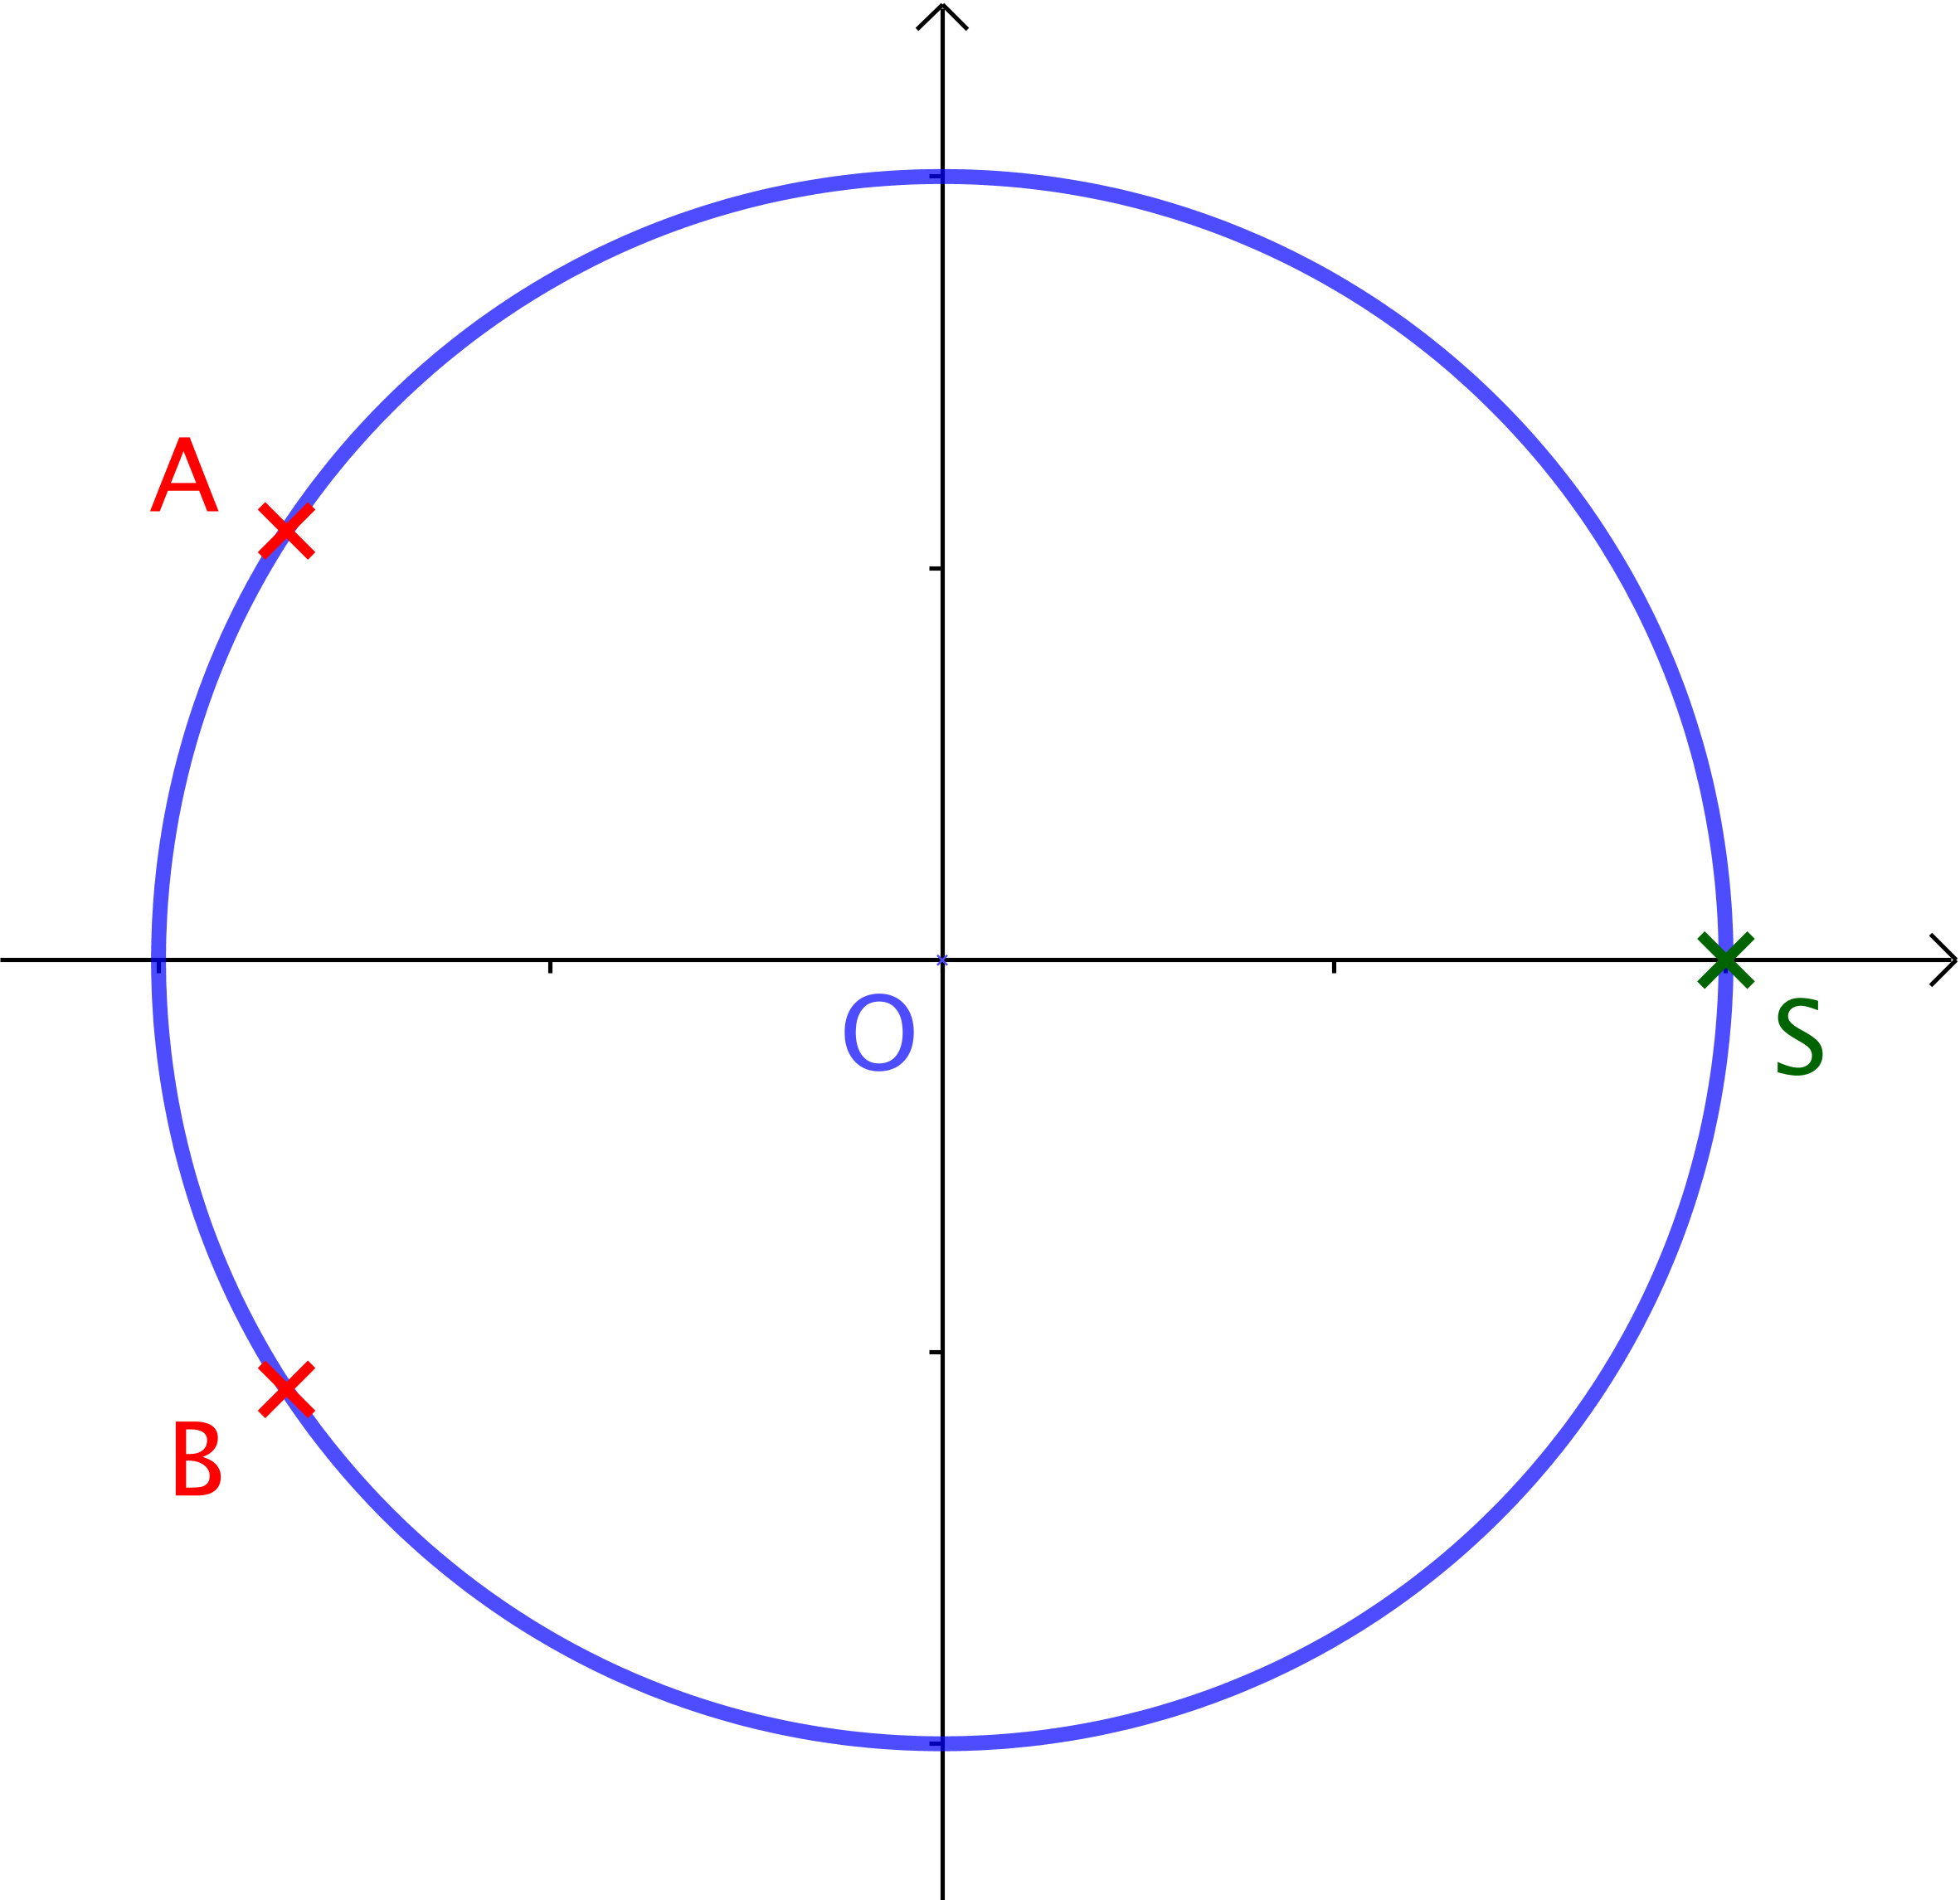
\includegraphics[scale = .75]{addition-on-ellipsis/conjecture/h-sym.png}}

	\columnbreak

	\fbox{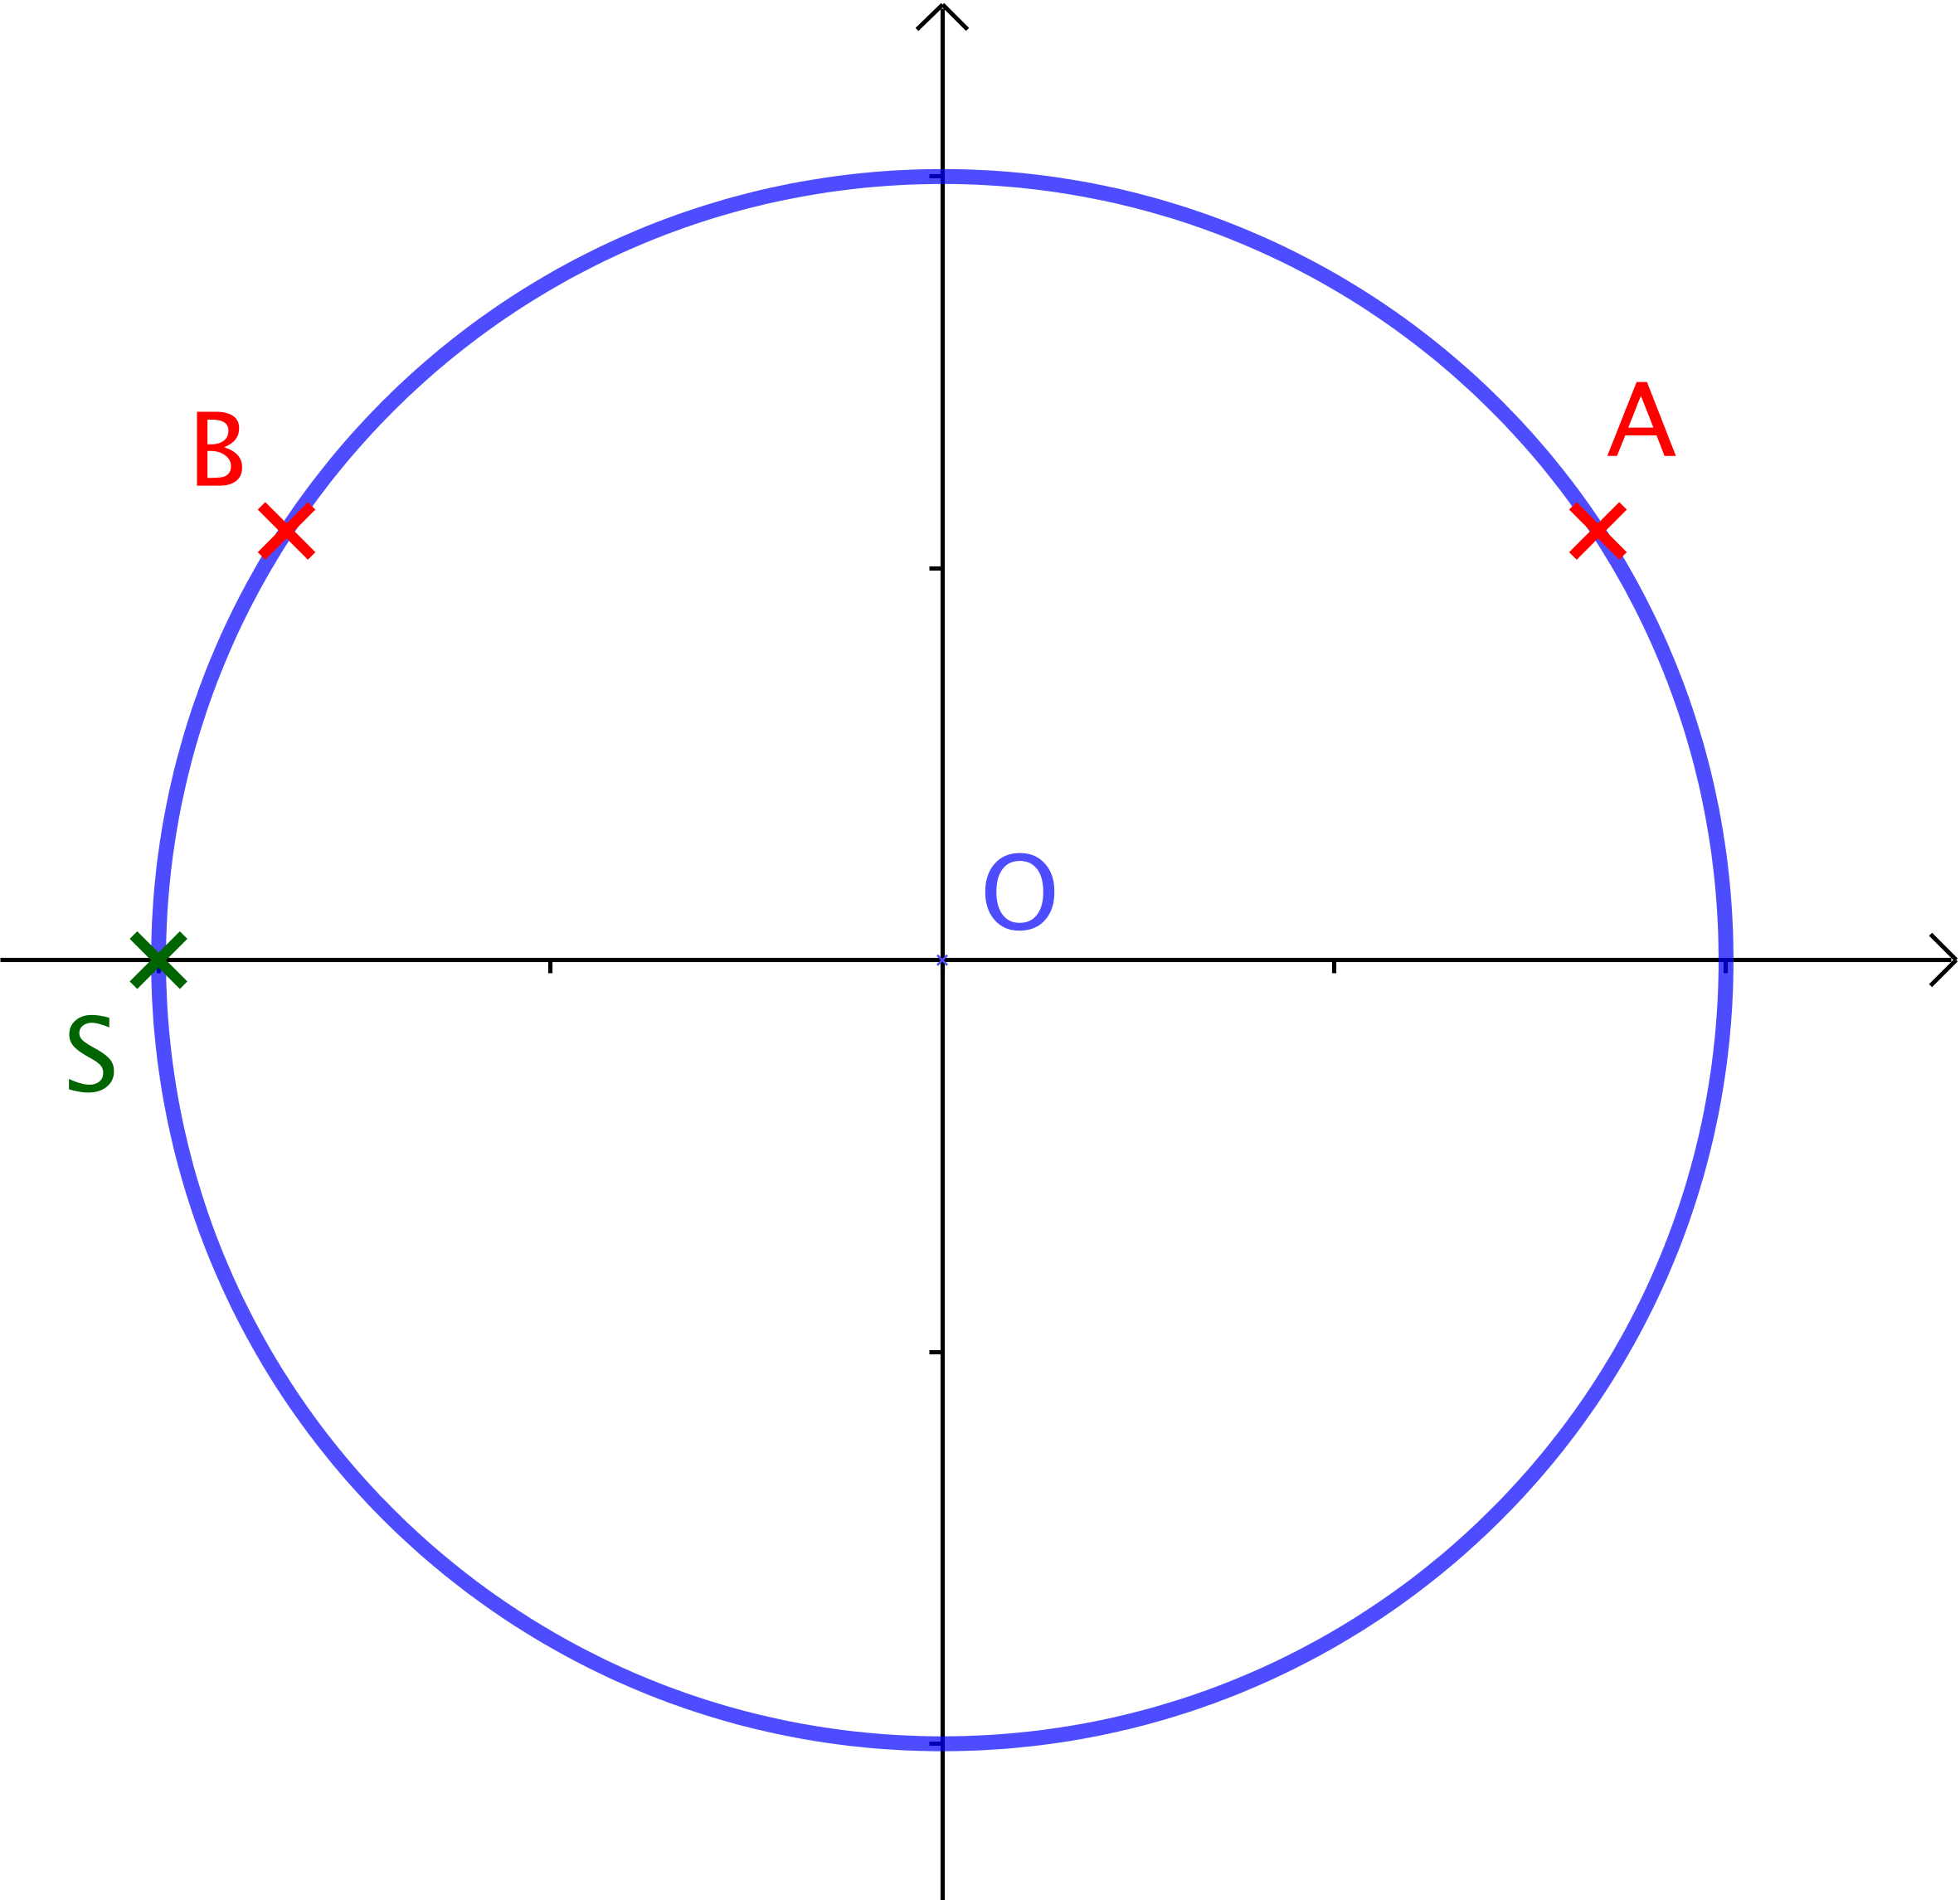
\includegraphics[scale = .75]{addition-on-ellipsis/conjecture/v-sym.png}}
\end{multicols}


\medskip

\begin{multicols}{2}
	\center

	\fbox{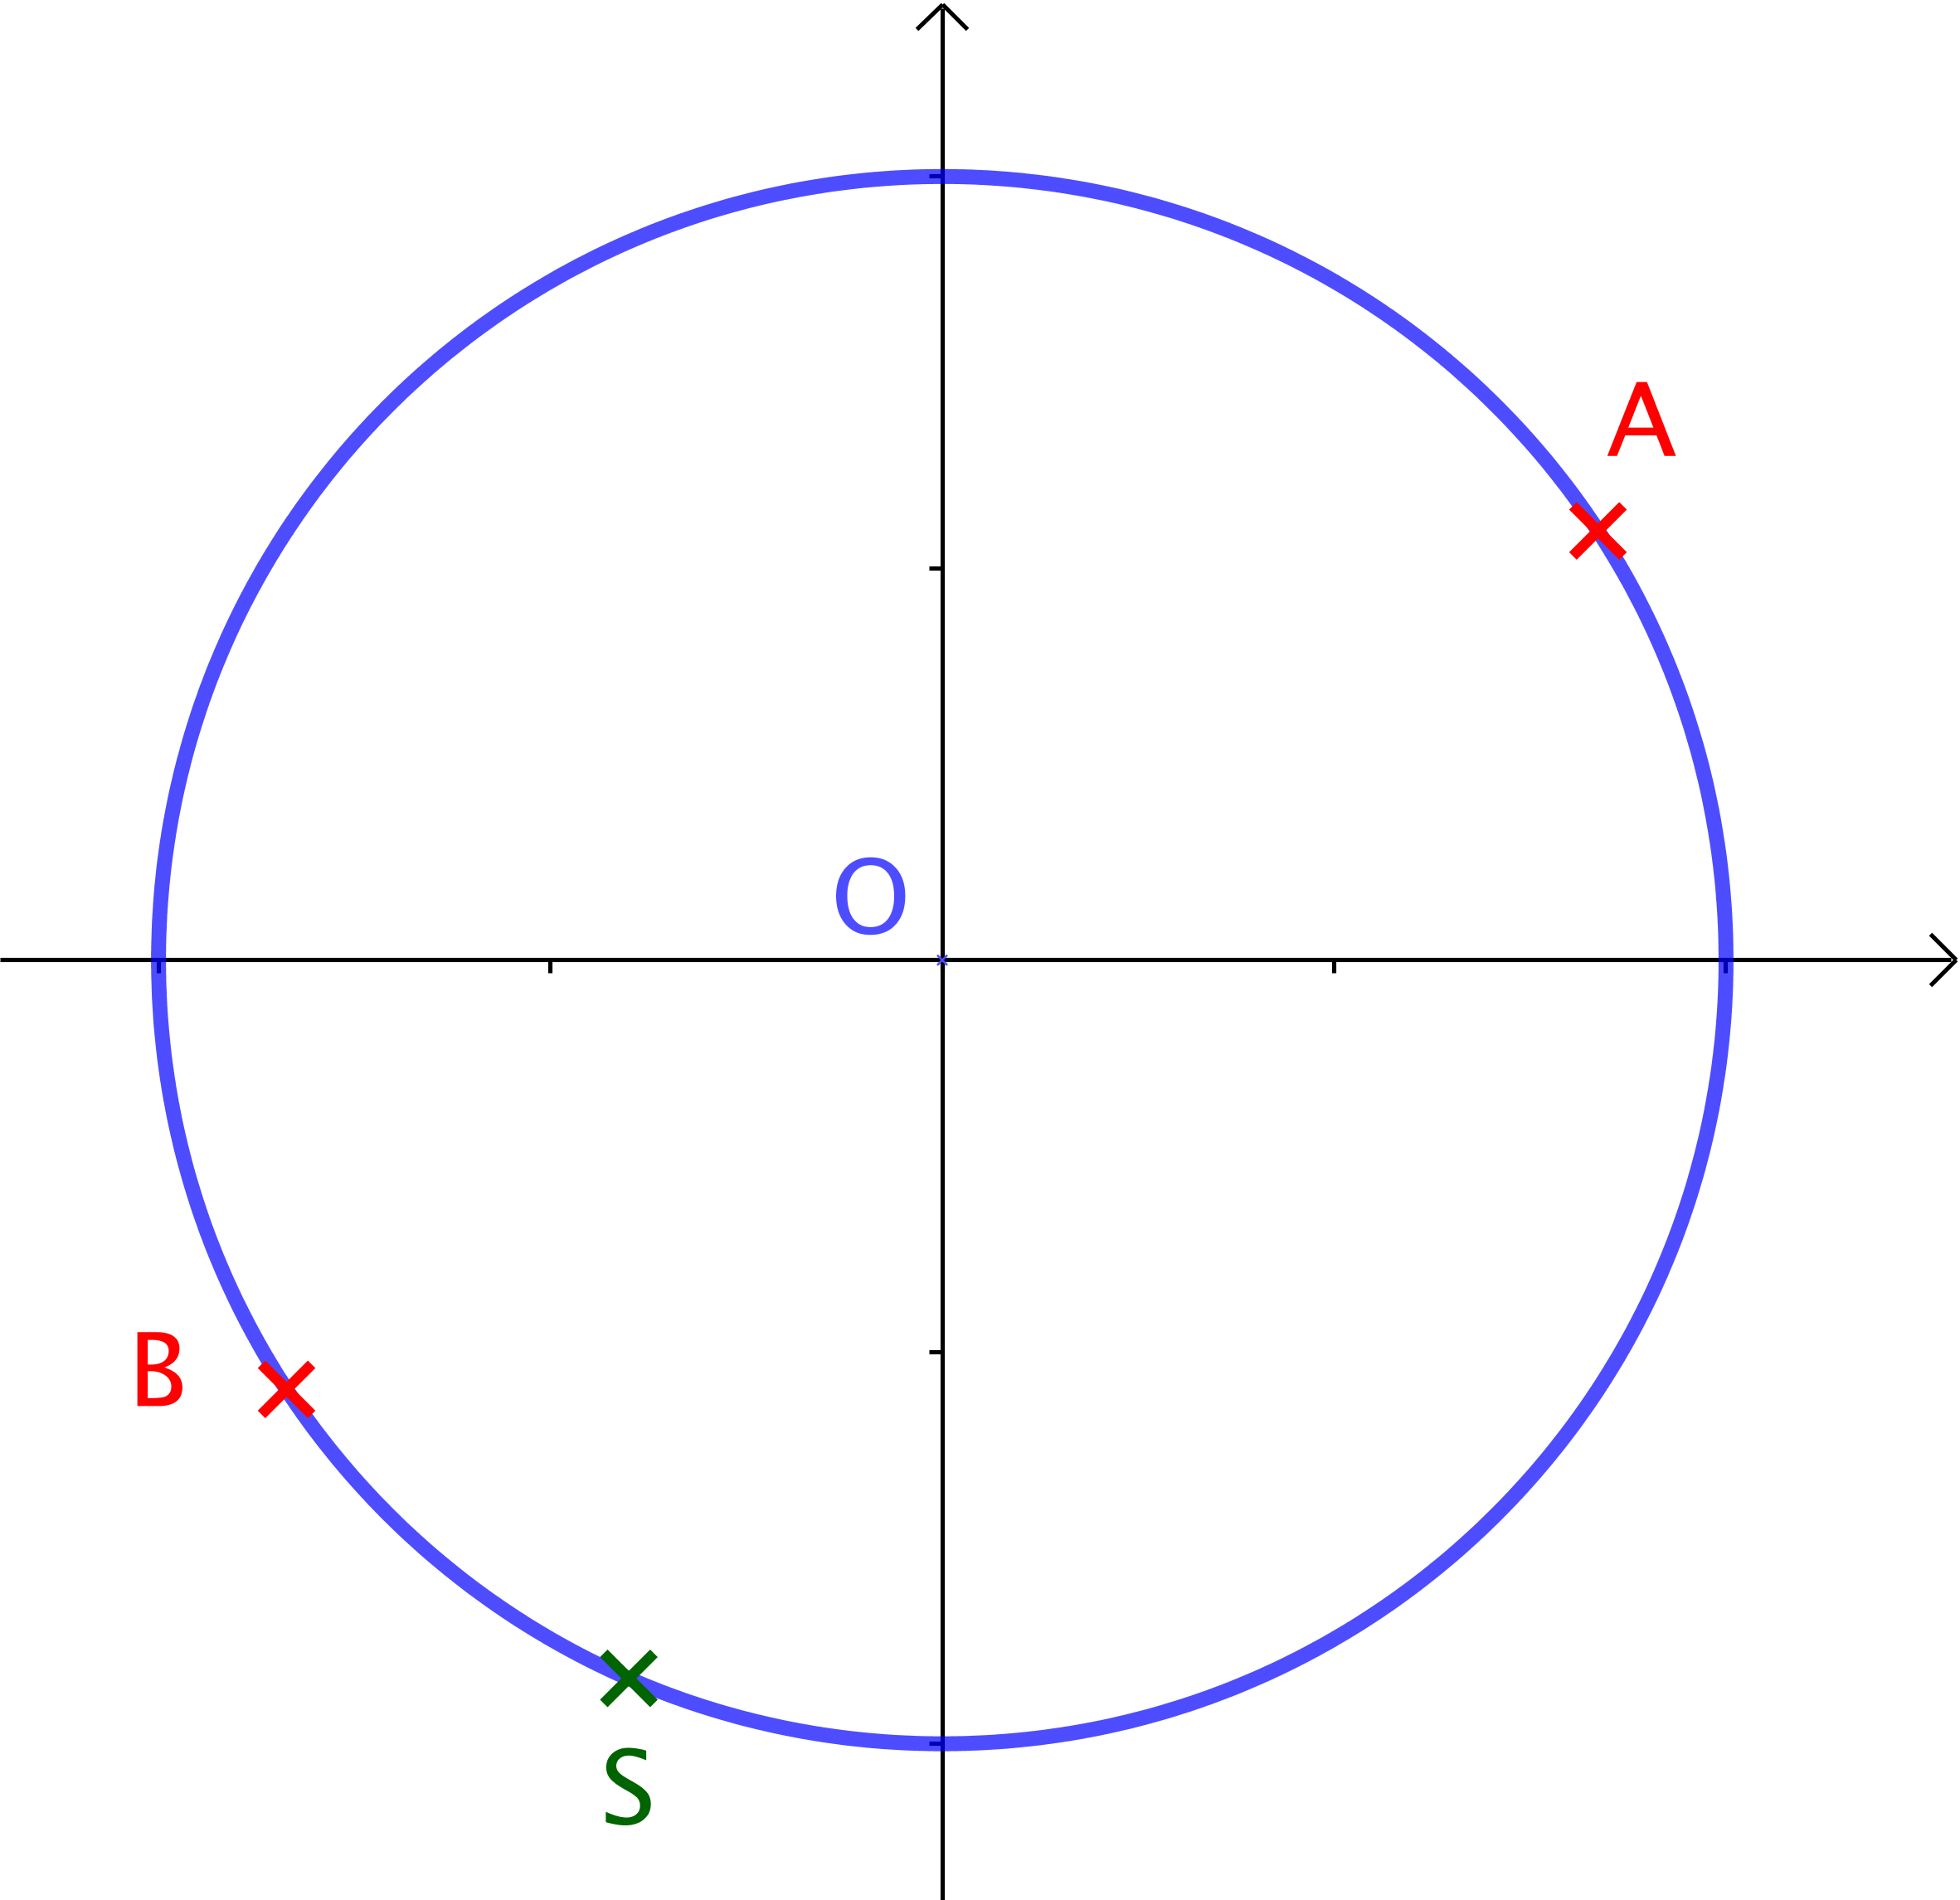
\includegraphics[scale = .75]{addition-on-ellipsis/conjecture/O-sym.png}}

	\columnbreak

	\fbox{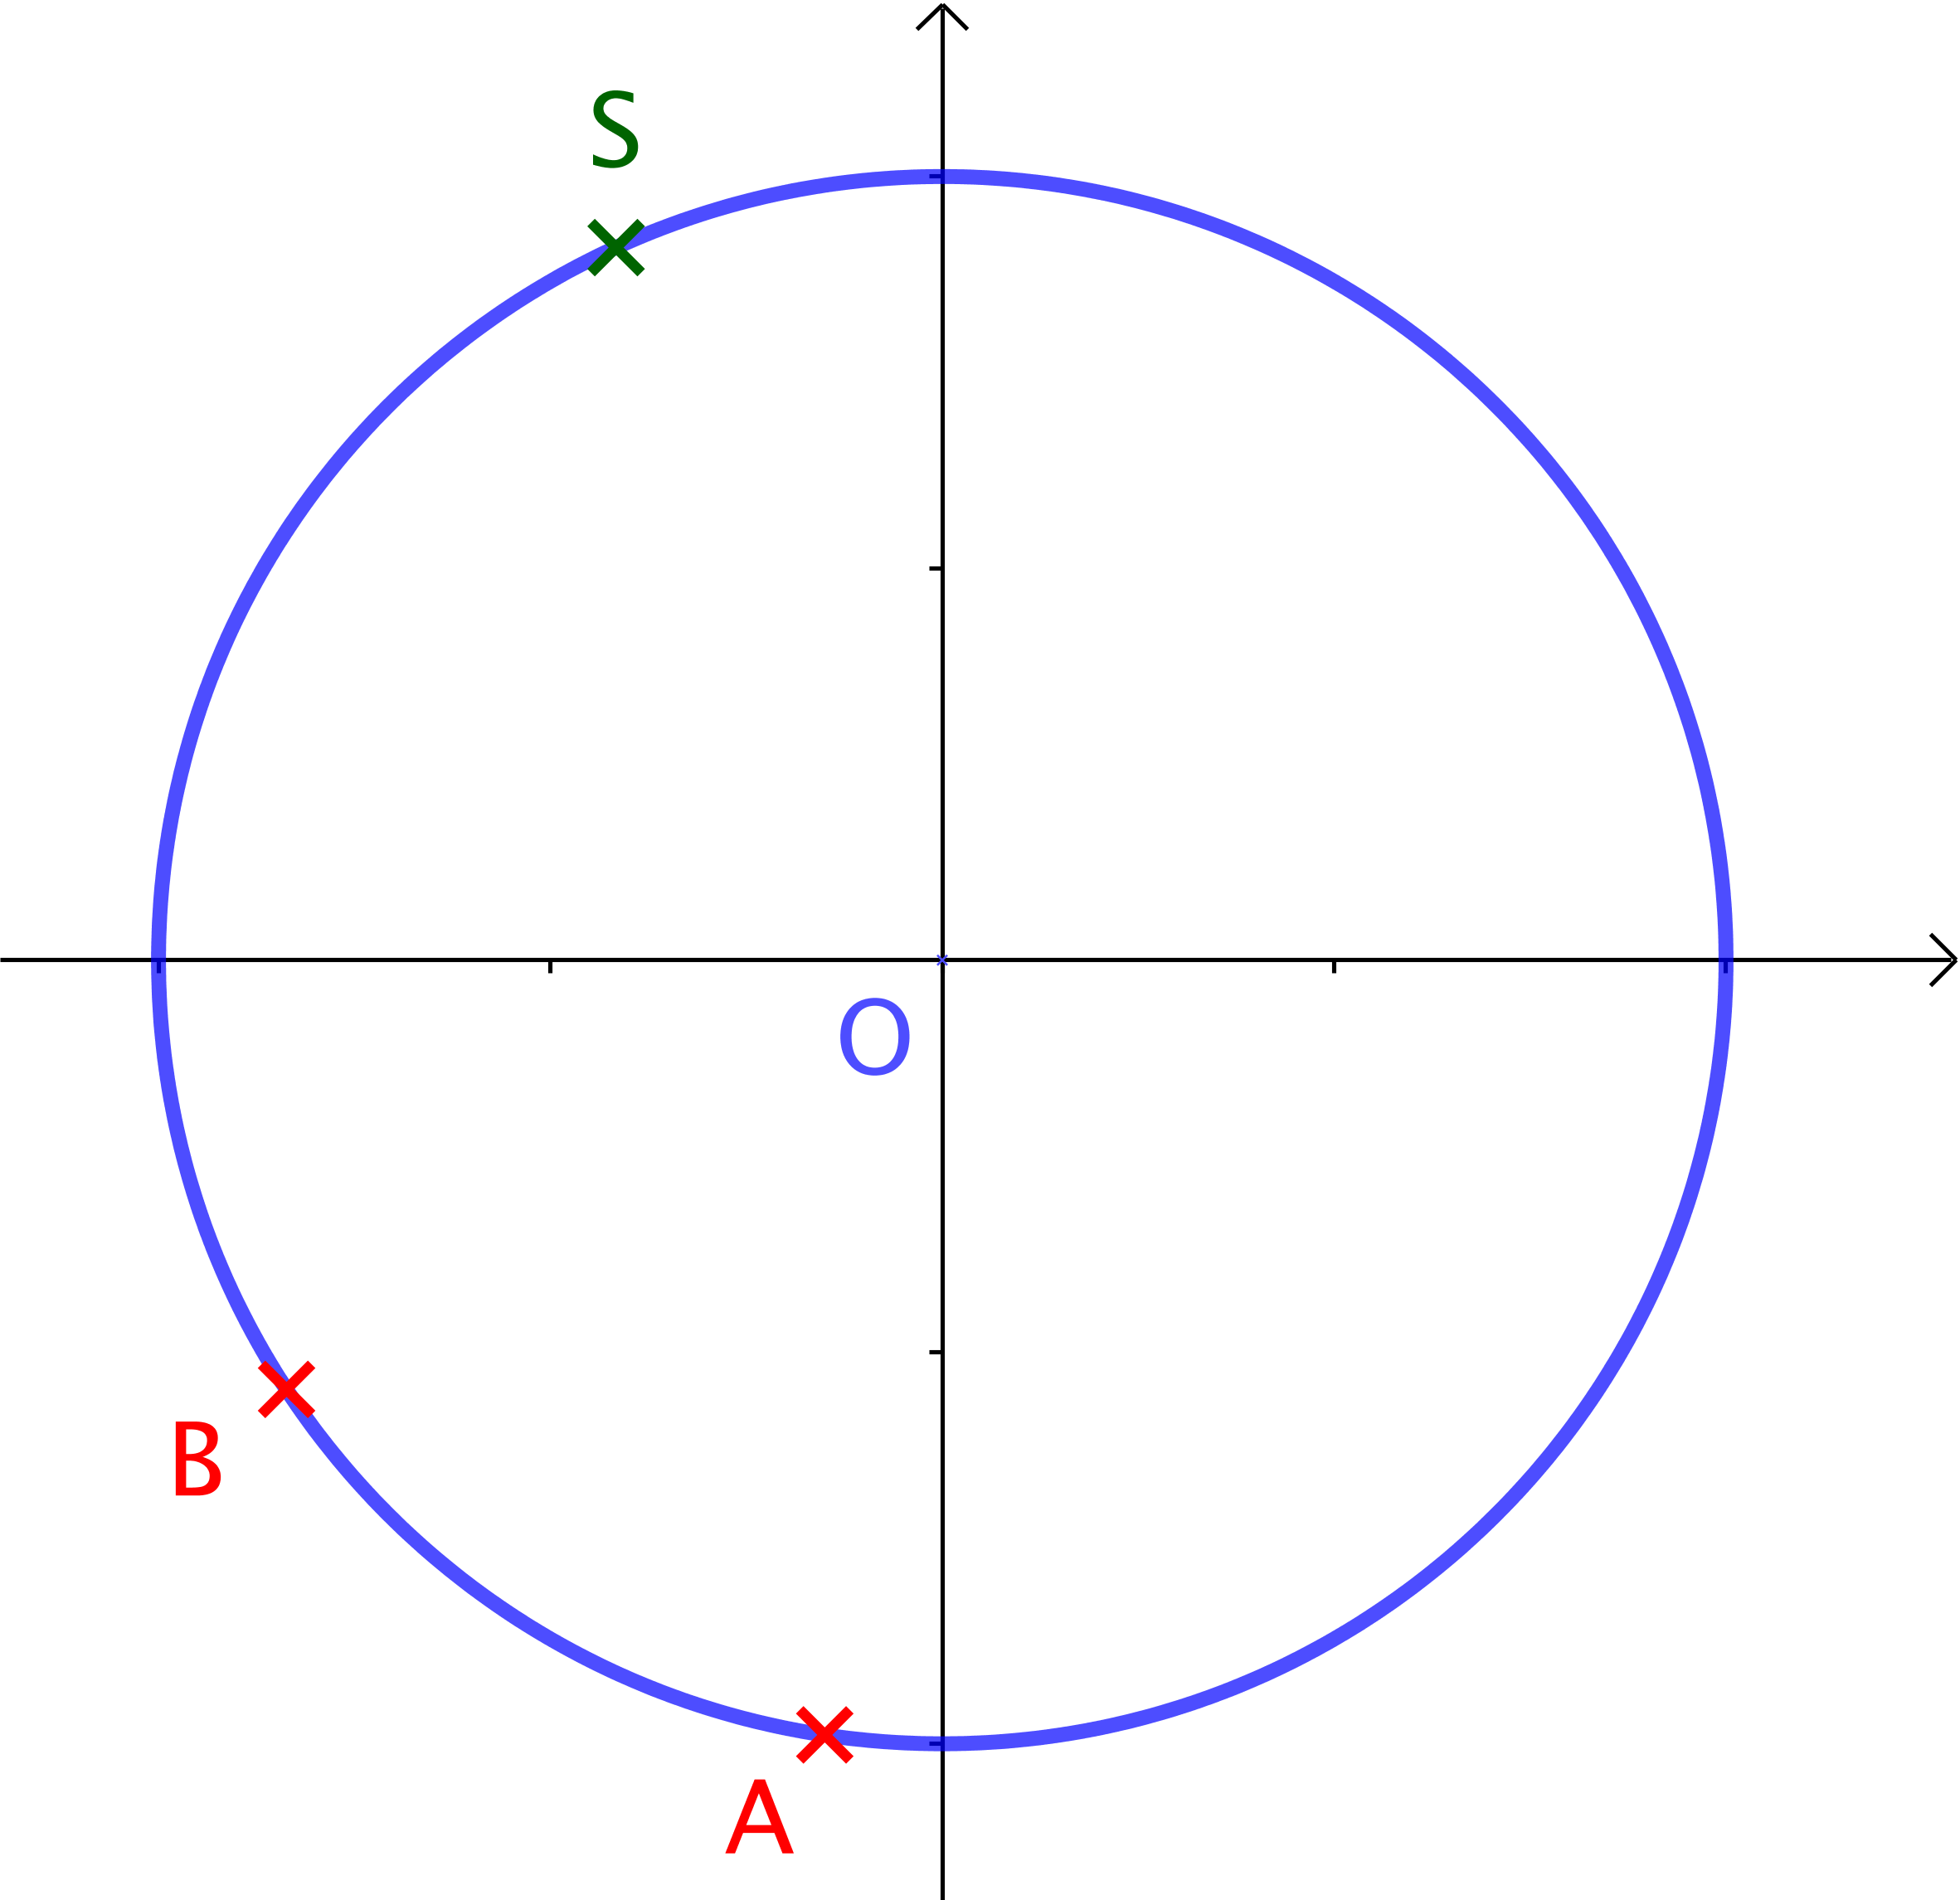
\includegraphics[scale = .75]{addition-on-ellipsis/conjecture/general.png}}
\end{multicols}


\newpage

Pour mieux voir ce qu'il se passe, il suffit de tracer quelques droites. Voici ce que cela donne.

\begin{multicols}{2}
	\center

	\fbox{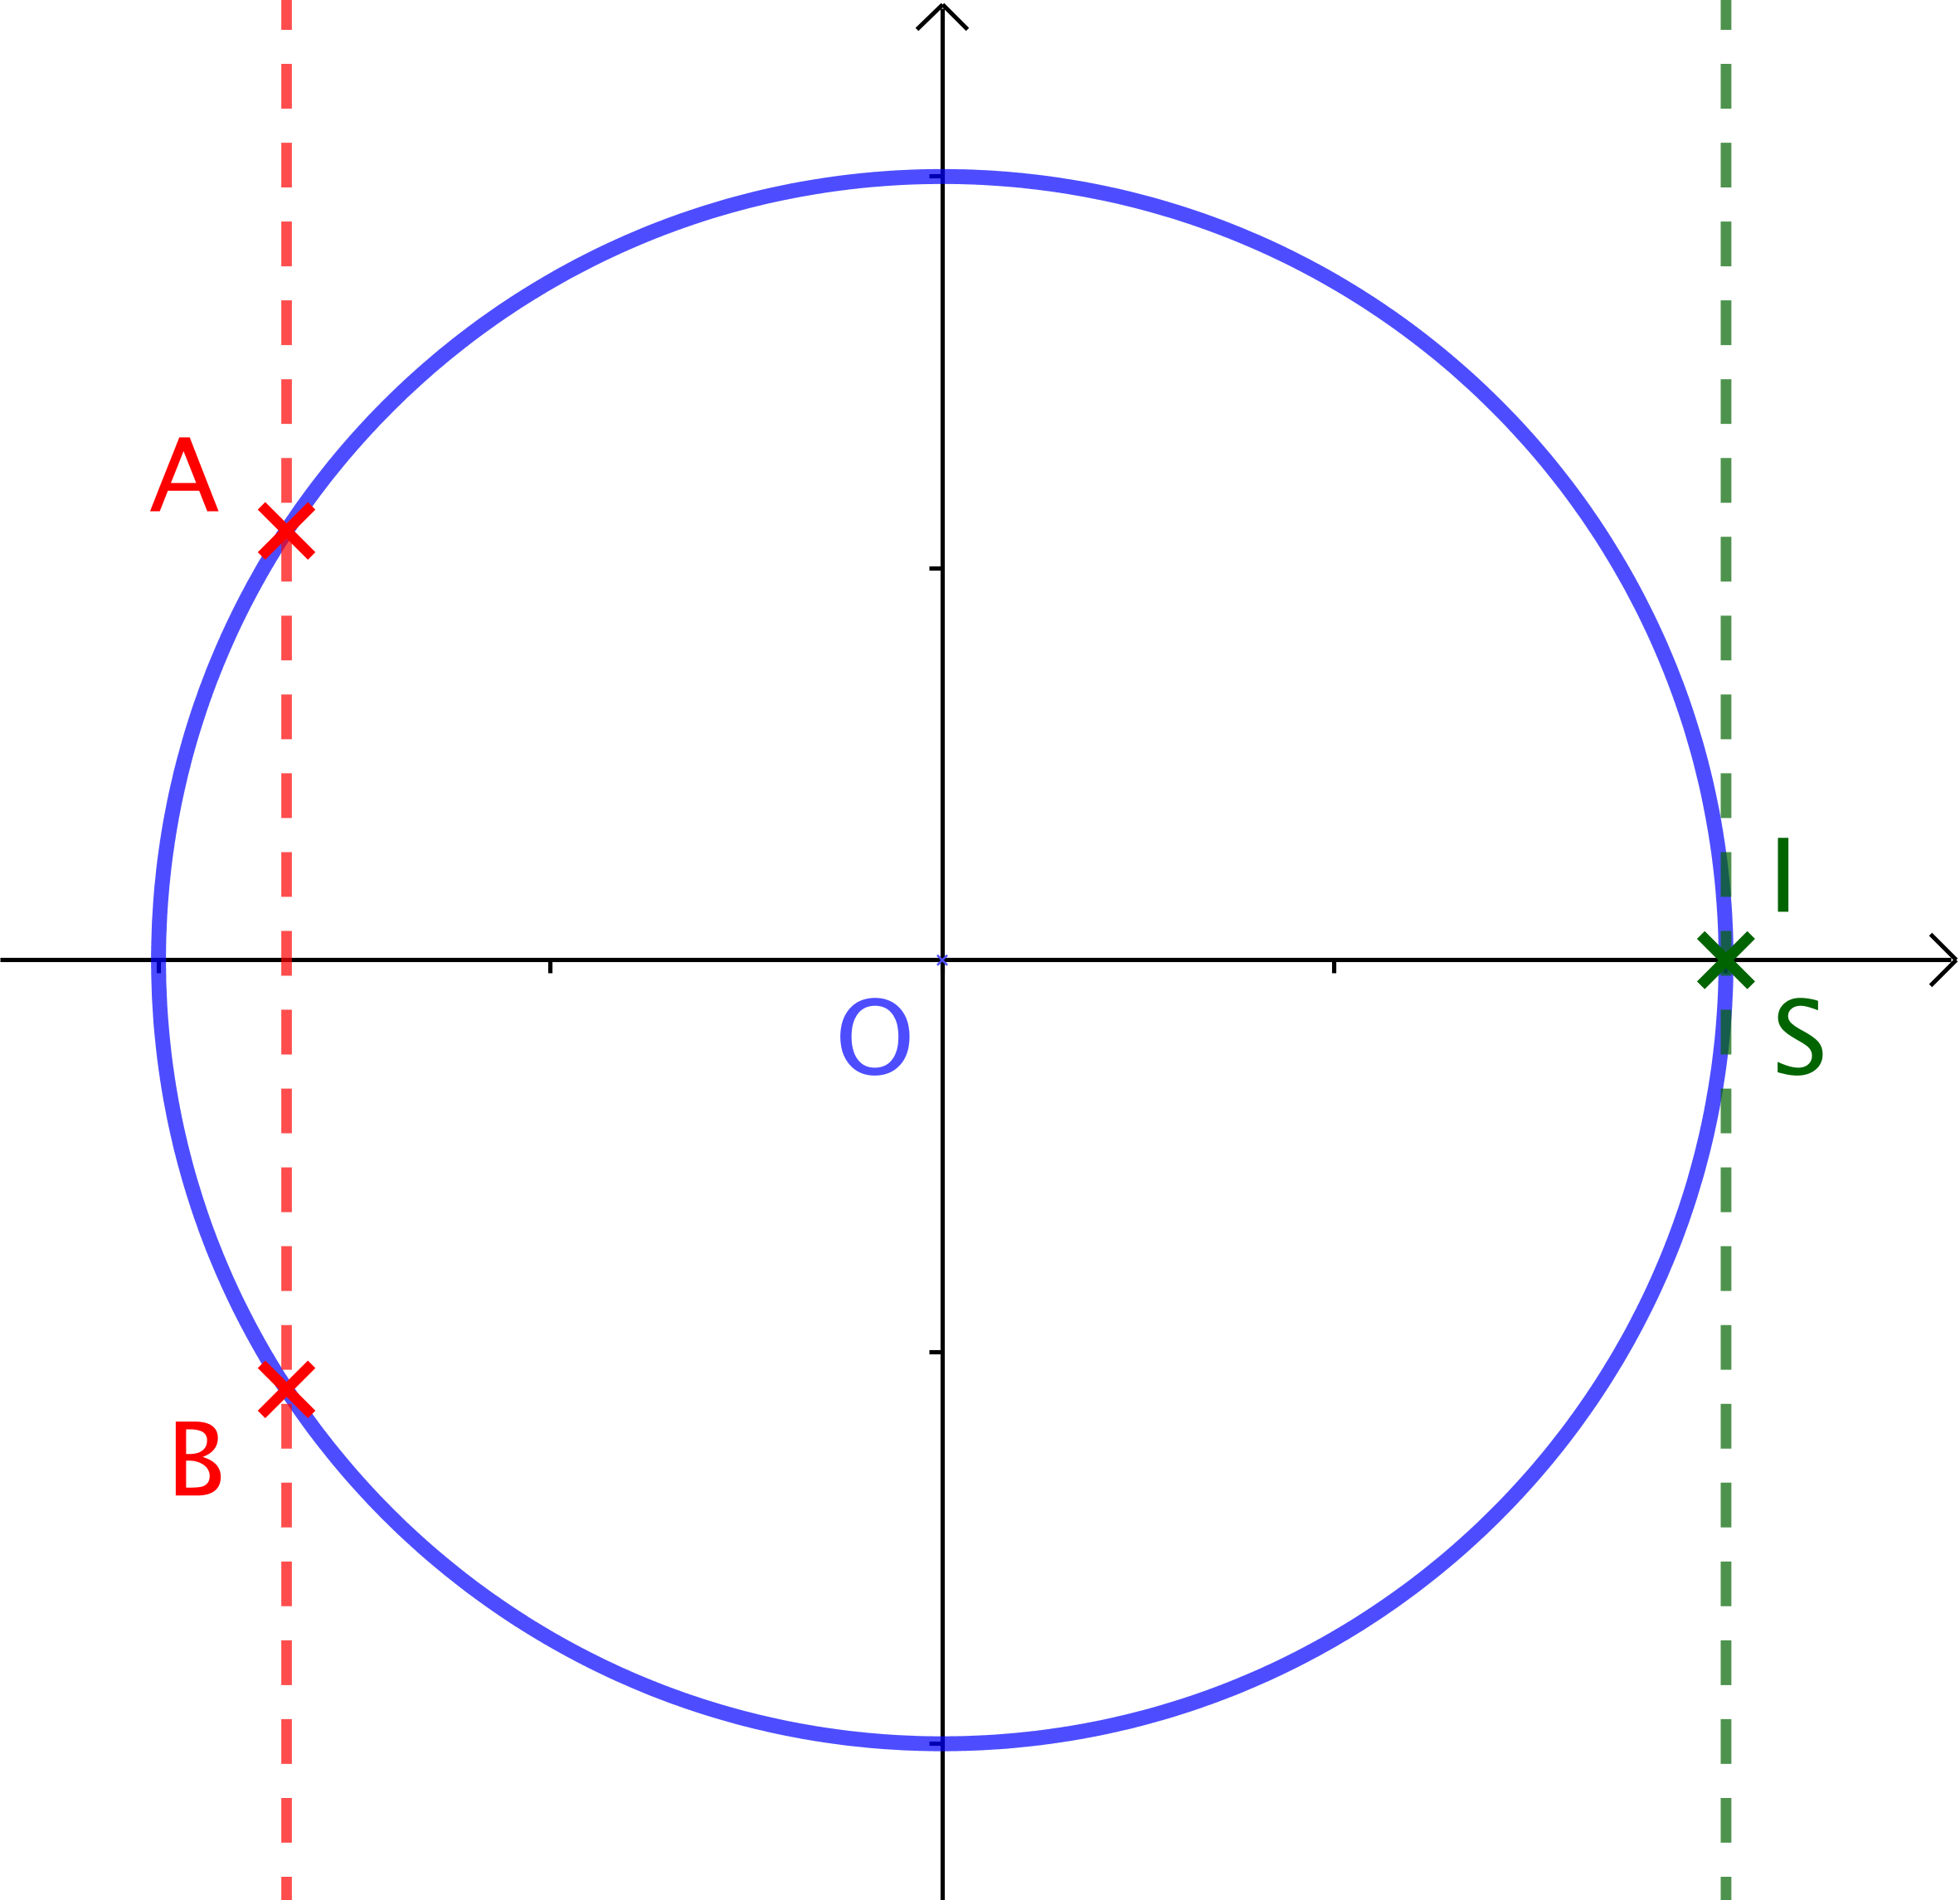
\includegraphics[scale = .75]{addition-on-ellipsis/conjecture/h-sym-with-lines.png}}

	\columnbreak

	\fbox{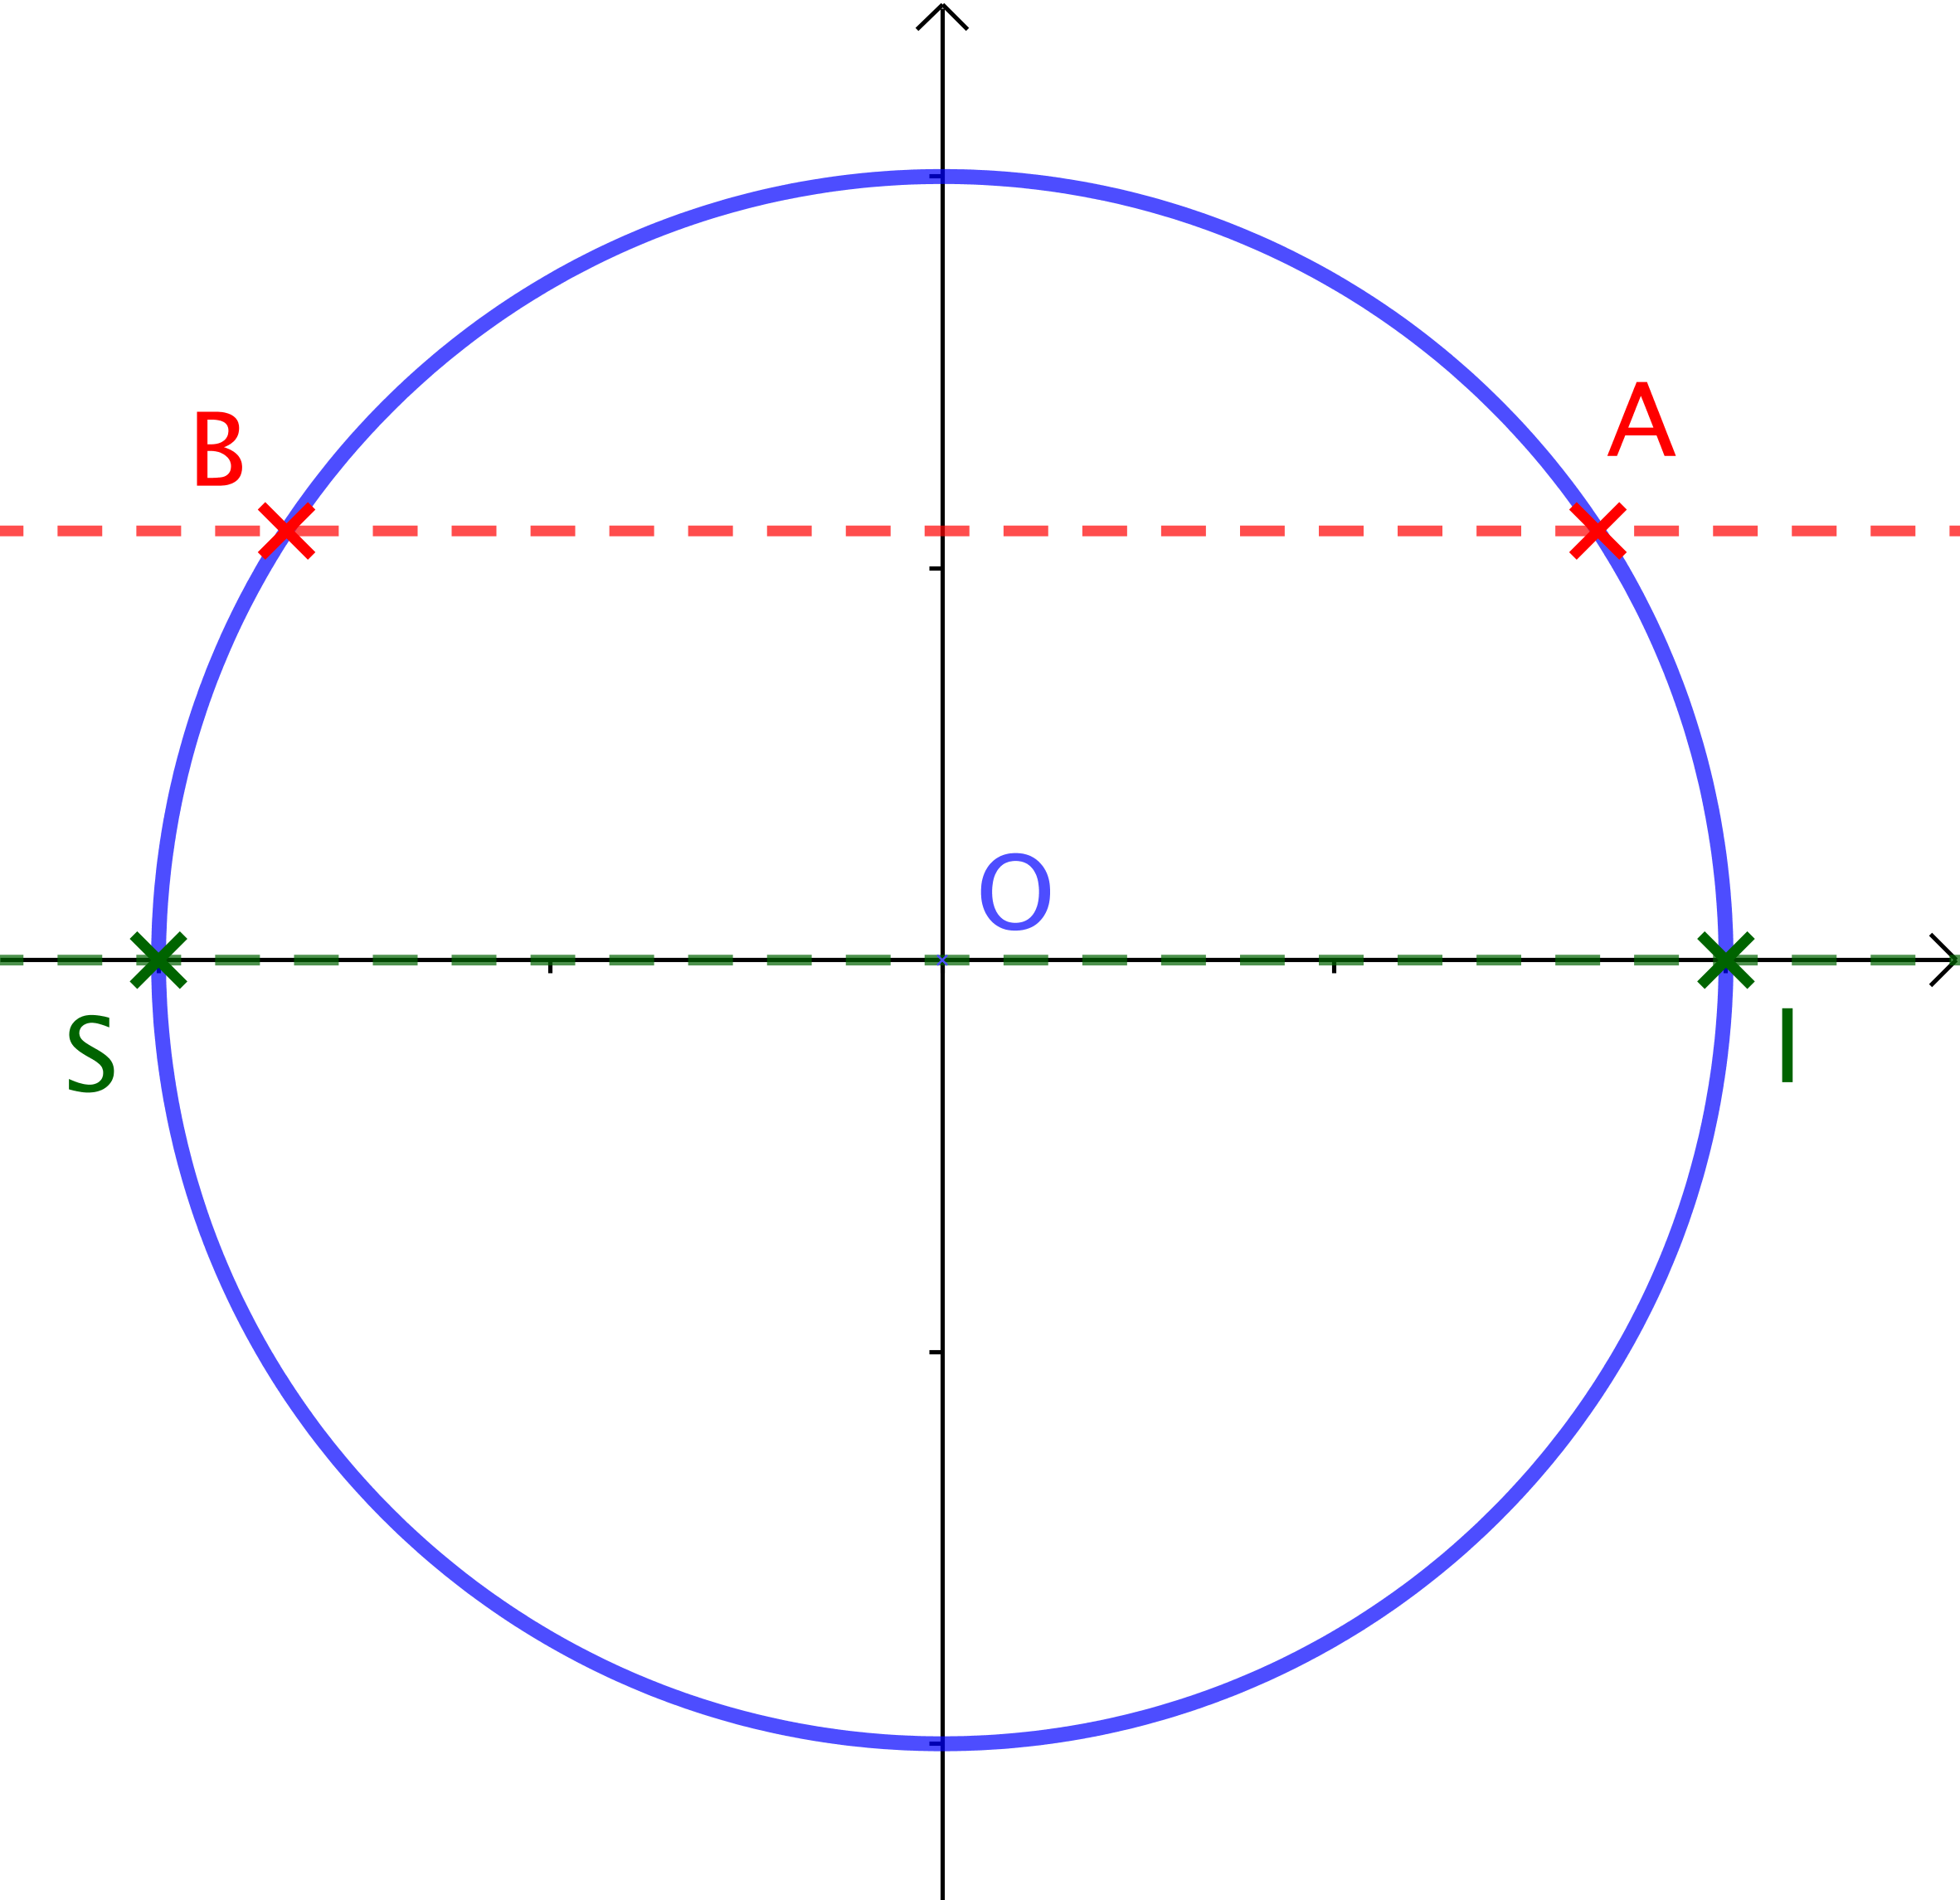
\includegraphics[scale = .75]{addition-on-ellipsis/conjecture/v-sym-with-lines.png}}
\end{multicols}


\medskip

\begin{multicols}{2}
	\center

	\fbox{\includegraphics[scale = .75]{addition-on-ellipsis/conjecture/o-sym-with-lines.png}}

	\columnbreak

	\fbox{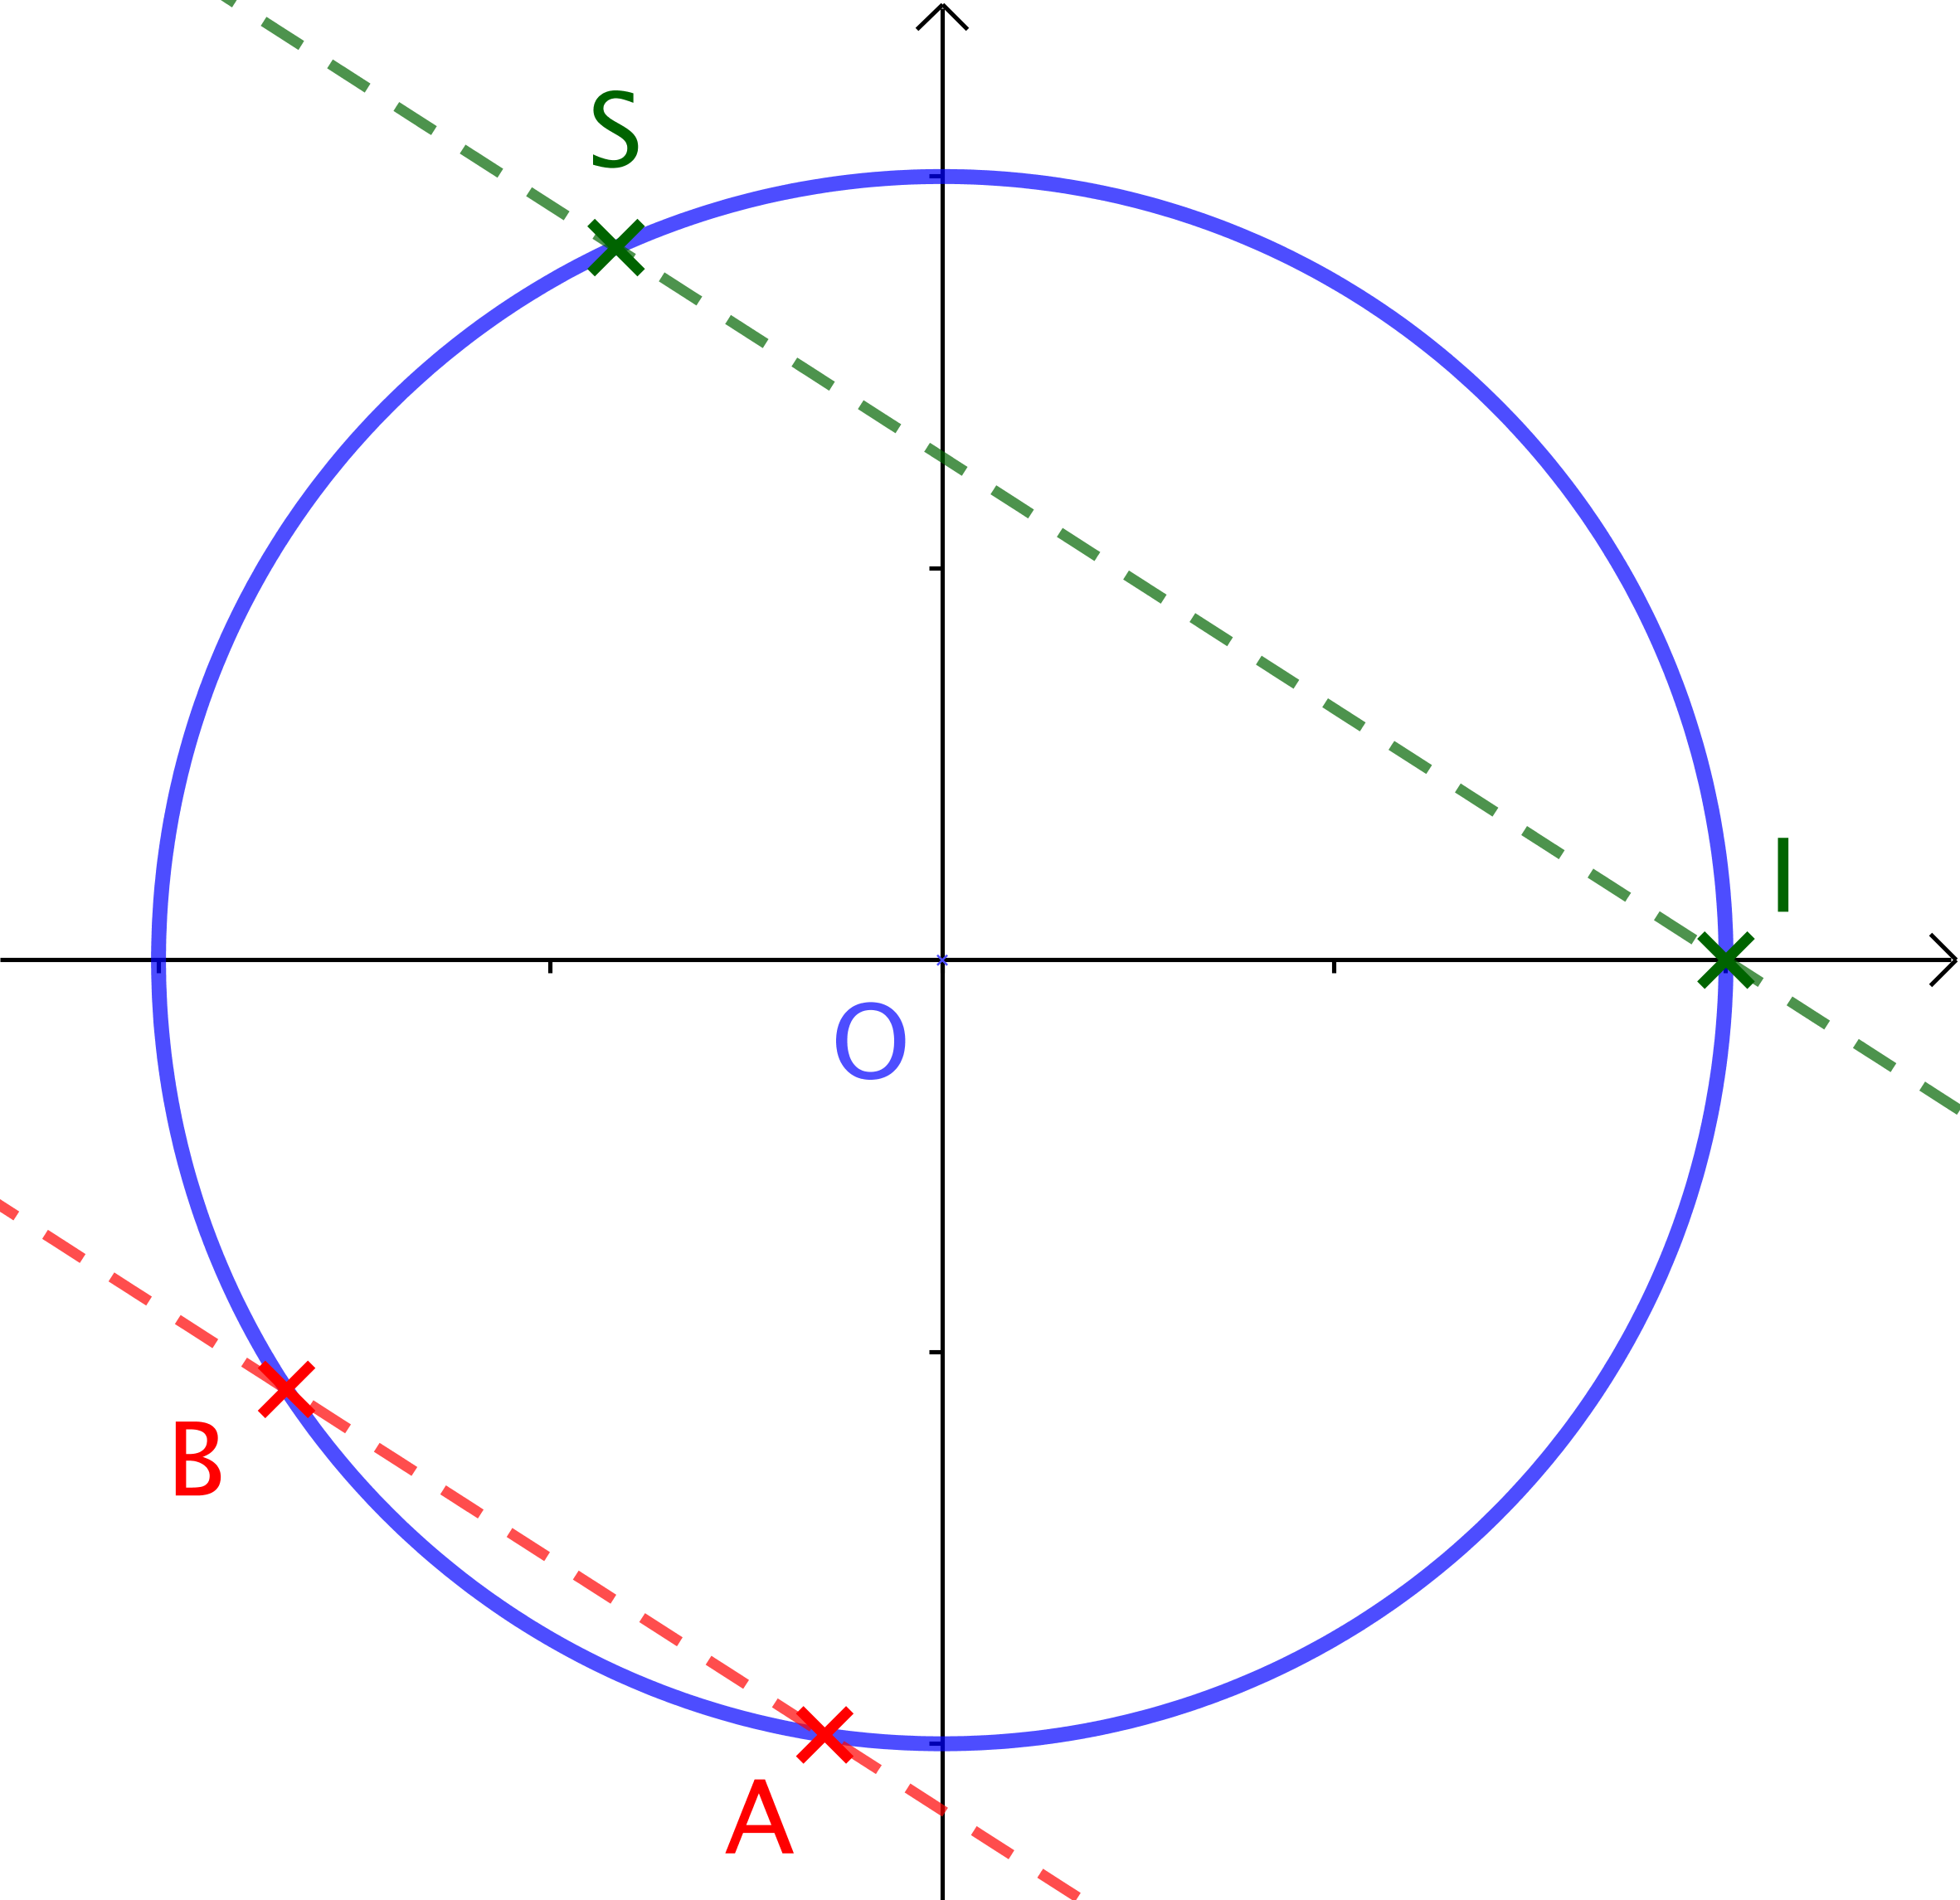
\includegraphics[scale = .75]{addition-on-ellipsis/conjecture/general-with-lines.png}}
\end{multicols}


Il devient évident de conjecturer que le point $S$ se construit géométriquement comme suit.

\begin{enumerate}
	\item \label{point-1} Si $A \neq B$ alors on construit la parallèle à $(AB)$ passant par $I$ . 
	Si cette parallèle n'est pas tangente au cercle alors le point $S$ est le second point d'intersection de cette parallèle avec le cercle, sinon $S = I$ .
	Notons que dans le second cas, c'est à dire si $x_A = x_B$ et $y_A = -y_B$ , alors $S = I$ peut être vu comme un point d'intersection \squote{double}.

	\item Si $A = B$ , on procède comme au point (\ref{point-1}) mais avec la parallèle à la tangente en $A$ au cercle. Intuitivement, cette situation consiste à faire \emph{\og tendre \fg} $A$ vers $B$ 
	\footnote{
		Nous évitons les arguments faisant appel à l'analyse afin de rester dans un cadre géométrique le plus général possible.
	}.
\end{enumerate}


\medskip

Dans ce qui suit nous allons valider cette conjecture de trois façons en allant du plus brutal au plus élégant.

\begin{enumerate}
	\item La 1\iere{} méthode passe assez brutalement via les critères de colinéarité et d'orthogonalité dans un plan.
	
	\item La 2\ieme{} méthode utilise les nombres complexes avec des calculs faciles à mener.
	
	\item La 3\ieme{} méthode, sûrement la plus élégante, est purement géométrique.
\end{enumerate}




\section{Preuve de la validité de la conjecture} \label{proof}

Rappelons que $\setgeo{H} : y = \frac{1}{x}$ , $E(1 ; 1)$ , $A \left( a ; \frac{1}{a} \right)$ , $B \left( b ; \frac{1}{b} \right)$ et $P \left( p ; \frac{1}{p} \right)$ où $p = a b$ avec $(a ; b) \in \left( \RRs \right)^2$ .



\bigskip

\textbf{Cas 1.} \emph{Supposons que $x_A x_B = 1$ .}

\medskip

Il est clair que $P = E$ dans ce cas.



\bigskip

\textbf{Cas 2.} \emph{Supposons que $x_A x_B \neq 1$ et $A \neq B$ .}

\medskip

La droite $(AB)$ a pour pente
$\frac{y_A - y_B}{x_A - x_B} = \frac{1}{a - b} \left( \frac{1}{a} - \frac{1}{b} \right) = - \frac{1}{ab}$ .
De plus, la droite $(EP)$ , qui existe car $p \neq 1$ , a pour pente
$\frac{y_P - y_E}{x_P - x_E} = \frac{1}{p - 1} \left( \frac{1}{p} - 1 \right) = - \frac{1}{p} = - \frac{1}{ab}$ .
Les droites $(AB)$ et $(EP)$ sont bien parallèles comme nous l'avons affirmé.



\bigskip

\textbf{Cas 3.} \emph{Supposons que $x_A x_B \neq 1$ et $A = B$ .}

\medskip

Comme ici $p = a^2 \neq 1$ . la droite $(EP)$ a pour pente $\left( - \frac{1}{a^2} \right)$ qui est aussi la pente de la tangente en $A \left( a ; \frac{1}{a} \right)$ à l'hyperbole $\setgeo{H}$ comme annoncé. 



\section{\texorpdfstring{Toute hyperbole d'équation $y = \frac{a x + b}{c x + d}$ a une structure de groupe}%
                        {Toute hyperbole d'équation y = (a x + b) / (c x + d) a une structure de groupe}}
      
Dans les preuves des sections précédentes, on constate que la construction géométrique se traduit par une identité basique qui est la clé de la périodicité de la suite de points $\left( A_i \right)$ . 
\begin{enumerate}
	\item Pour le cercle, c'était $\theta_i + \theta_{i+1} = \theta_{i+3} + \theta_{i+4}$ avec $\theta_i = \vangleorient{OI}{OA_i}$ . Nous nous intéressons ici juste à la 2\ieme preuve donnée dans la section \ref{circle-proof-2}. 

	\item Pour la parabole, c'était $x_i + x_{i+1} = x_{i+3} + x_{i+4}$ avec $x_k \in \RR$ des abscisses. 

	\item Pour l'hyperbole, c'était  $x_i x_{i+1} = x_{i+3} x_{i+4}$ avec $x_k \in \RRs$ des abscisses.
\end{enumerate}


\medskip


En fait, si $\Gamma$ désigne une ellipse, une parabole quelconque, ou une hyperbole quelconque, on peut démontrer l'existence d'un point $E \in \Gamma$ tel que la construction qui à $A \in \Gamma$ et $B \in \Gamma$ associe le point $S$ tel que $\setgeo*{C}{AB} \,/\!/\, \setgeo*{C}{ES}$ définisse une loi de groupe $\star$ sur $\Gamma$ avec $E$ pour élément neutre. 
Les cas étudiés dans ce document n'en sont que des cas particuliers. 
Le lecteur intéressé peut se reporter à  
\emph{\og Faire des additions modulaires sur une ellipse \fg} ,
\emph{\og Faire des additions sur une parabole \fg} 
et
\emph{\og Faire des produits sur une hyperbole \fg}
qui ont été rédigés par l'auteur de ce document
\footnote{
	Voir \texttt{addition-on-ellipsis.pdf} , \texttt{addition-on-parabolas.pdf}  et \texttt{product-on-hyperbolas.pdf}  à l'adresse \url{https://github.com/bc-writing/drafts} .
}.


\medskip


Tout comme dans la preuve dans la section \ref{circle-proof-2} , on constate alors que la construction \emph{\og magique \fg} est telle que $\forall n \in \NN_{\geq 5}$ , $A_{n}$ est l'unique point de $\Gamma$ tel que $\setgeo*{C}{A_{n} A_{n-1}} \,/\!/\, \setgeo*{C}{A_{n-3} A_{n-4}}$ . On en déduit alors que $A_{n} \star A_{n-1} = A_{n-3} \star A_{n-4}$ . On retombe alors sur une identité similaire à celles redonnées ci-dessus mais avec la loi $\star$ au lieu des lois $+$ avec des angles orientés, $+$ avec des réels et $\times$ avec des réels non nuls. On conclut alors de la même façon. Que les mathématiques sont belles quand on prend le temps de les écouter !




% Voir si caractéristique : il transof complexe de 1/x vers x^2 uis on utiliserait cas complexe pour revenir à l'hyperbole . FAISABLE ???????
\end{document}
